\documentclass{article}
\usepackage{amsmath}    % For math mode and the pmatrix environment
\usepackage{tikz}       % For drawing the lines
\usetikzlibrary{calc}   % Needed for relative coordinate calculations

% Define custom colors
\definecolor{myred}{RGB}{200,0,0}
\definecolor{mygreen}{RGB}{0,150,0}

% Define TikZ styles for the arrows (changed to 'thin')


\begin{document}
\[\begin{pmatrix}
        5 & 2 & 4 & 5 & 2 \\
        1 & 3 & 8 & 1 & 3 \\
        7 & 9 & 6 & 7 & 9
    \end{pmatrix}\]
\begin{equation*} % Use equation* for centering without a number
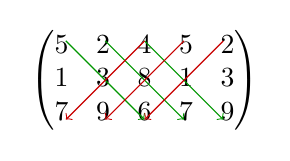
\begin{tikzpicture}[
    % Global settings for nodes (numbers)
    every node/.style={
        minimum width=1em, 
        inner sep=0.1em,     
        font=\normalsize,
    },
    % Positioning of the matrix elements (smaller spacing)
]

\node (M) at (0, 0) {
    $\begin{pmatrix}
        5 & 2 & 4 & 5 & 2 \\
        1 & 3 & 8 & 1 & 3 \\
        7 & 9 & 6 & 7 & 9
    \end{pmatrix}$
};
\tikzset{
    red_arrow/.style={->, myred, thin},
    green_arrow/.style={->, mygreen, thin}
}
\pgfmathsetmacro{\colwidth}{1}
\pgfmathsetmacro{\rowheight}{2}

\draw[green_arrow] (-1,0.5) -- (0,-0.5); 
\draw[green_arrow] (-0.5,0.5) -- (0.5,-0.5);
\draw[green_arrow] (0,0.5) -- (1,-0.5);

\draw[red_arrow] (0,0.5) -- (-1,-0.5); 
\draw[red_arrow] (0.5,0.5) -- (-0.5,-0.5); 
\draw[red_arrow] (1,0.5) -- (0,-0.5); 

\end{tikzpicture}
\end{equation*}

\end{document}